%%%%%%%%%%%%%%%%%%%%%%%%%%%%%%%%%%%%%%%%%%%%%%%%%%%%%%%%%%%%%%%%%%% 
%                       rpithes-short.tex                         %
%         Template for a short thesis all in one file             %
%        (titlepage info below assumes masters degree}            %
%  Just run latex (or pdflatex) on this file to see how it looks  %
%      Be sure to run twice to get correct TOC and citations      %
%%%%%%%%%%%%%%%%%%%%%%%%%%%%%%%%%%%%%%%%%%%%%%%%%%%%%%%%%%%%%%%%%%% 
%
%  To produce the abstract title page followed by the abstract,
%  see the template file, "abstitle-mas.tex"
%
%%%%%%%%%%%%%%%%%%%%%%%%%%%%%%%%%%%%%%%%%%%%%%%%%%%%%%%%%%%%%%%%%%%

\documentclass{thesis}
\usepackage{graphicx}   % if you want to include graphics files
\graphicspath{{../images/}}


\usepackage[draft]{todonotes}

\newcommand{\comment}[1]
{\par {\bfseries \color{blue} #1 \par}} %comment showed

% Use the first command below if you want captions over 1 line indented.
% A side effect of this is to remove the use of bold for captions. 
% To restore bold, also include the second line below.
%\usepackage[hang]{caption}     % to indent subsequent lines of captions
%\renewcommand{\captionfont}{\bfseries} % only needed with caption package;
                                        %   otherwise bold is default)


%%%%%%%%%%%%%%%%%%%%  supply titlepage info  %%%%%%%%%%%%%%%%%%%%%
\thesistitle{\bf Federating AMQP1.0 Message-oriented Middleware (MOM) brokers}        
\author{David Joe Wade}        
\degree{Master of Science}
\department{Computer Science} 
\projadviser{Dr. Eugene Eberbach}
%  For a masters project use \projadviser instead of \thadviser, 
%  and \coprojadviser and \cocoprojadviser if needed. 
\submitdate{April 2014\\(For Graduation May 2014)}        

%%%%%%%%%%%%%%%%%%%%%   end titlepage info  %%%%%%%%%%%%%%%%%%%%%%
      
\begin{document} 
\listoftodos
\titlepage            	 % Print titlepage          
\tableofcontents          % required 
\listoftables          	 % required if there are tables
\listoffigures         	 % required if there are figures

\specialhead{ACKNOWLEDGMENT}
Special thanks to: my wife Anne, my son Jack, my daughter Erin, and my parents Brian and Catherine.  Thanks for letting me have the time to put this together!  

\specialhead{ABSTRACT}
Message passing is a fundamental aspect of systems engineering.  Without a methodology to pass information between separate components building a distributed system is impossible.  When building a distributed system it is very common for teams/organizations to develop proprietary message passing systems.  Because of their isolated development, these systems usually fill a very niche role and do not interoperate with other implementations. \footnote{Many middleware implementations that fail because of this - The author has specifically implemented two such systems in his professional career.  Both were replaced with other systems unused because of lack of interoperability.} This is a fundamental problem when trying to build larger systems from subsystems.  Without a common language and transport getting different components to communicate is difficult if not impossible.  There have been many attempts to develop a common languages and transports with varying amounts of success.  A new standard, developed by a consortium of large technology companies, the Advanced Message Queuing Protocol (AMQP) provides an open standard protocol for message orientated middleware (MOM).  There are currently several active AMQP compliant MOM implementations, both open-source and proprietary.  This project investigates the current state of several popular open-source AMQP message brokers, attempts to create a federated network of different implementations in order to collect benchmark information for both homogenous an heterogeneous broker networks.  To achieve this goal a simple AMQP messaging benchmark was developed and data collected from different broker architectures.  While it was possible to integrate some of the active broker implementations this project found that not all of the available implementations are interoperable and there are significant problems creating a reliable messaging system with all implementations.  

\chapter{INTRODUCTION}

\section{Middleware}
In computer science, the term \"middleware\" has many meanings.  Generically, middleware can be thought as \"glue\"  for computer software.  It facilitates communication between different software components - abstracting the complexities of intra and inter process communication from a software component.  In a broad sense many things that do clearly resemble a communication context are technically middleware.  User space software drivers, virtual machines (Java not VMware) and kernel Inter-process Communication (IPC) mechanisms are all forms of middleware.  This paper focuses on middleware as it relates to distributed applications - typically used to share data and state between software components.  Middleware at this level typically facilitates communication over a network and allows for components to work together in separate execution environments.  Even with this narrow definition there are many different classes of middleware systems.  Some of the common design patterns used are: enterprise application integration (EAI), data integration (DI), message-oriented middleware (MOM), object request brokers (ORB) and the enterprise service bus (ESB).  This paper specifically focuses on message-oriented middleware. 

\subsection{Message Oriented Middleware (MOM)}
Message-oriented middleware (MOM) is a middleware design that is focused on sending discrete blocks of information (messages) between processing components.  Messages can contain state information, commands or pure input data - it is up to the processing components to identify and process the messages according to their contents.  MOM systems are inherently asynchronous - processing components typically execute independently and are not synchronized to process in lockstep.

A fundamental component of MOM systems is a message broker.  A message broker is acts as an intermediary - all messages sent through a MOM system must be sent to a message broker.  A message broker performs many of the same functions as a network router on an ethernet network, but at a much higher level.  Message brokers can connect to either message producers, consumers or other message brokers - and are responsible for routing messages from the producer to consumer.  Frequently, message brokers are designed to do more than just route messages and are designed with the ability to store messages locally in order to provide message reliability.  Message brokers are often able to handle message duplication - that is to forward a message to multiple clients and provide for quality of service (QOS) to be applied to messages.  

While a message broker can provide many benefits, by adding an additional component between message producers and consumers this can reduce performance and reliability.  MOM systems also frequently require a significant amount of configuration to setup properly and add an extra layer of complexity when trying to debug a system.
 
%https://en.wikipedia.org/wiki/Message-oriented_middleware
%There are many implementations of such messaging systems, many are closed source proprietary, but recently there has been a lot of activity in the open source community.

\section{Advanced Message Queuing Protocol (AMQP)}
The Advanced Message Queueing Protocol (AMQP) is a standard published by the Organization for the Advancement of Structured Information Standards (OASIS) \cite{OASIS}.  In the Open Systems Interconnection (OSI) model AMQP is a application layer protocol, it exists in the same space as other protocols as the File Transfer Protocol (FTP), Dynamic Host Control Protocol (DHCP), etc.  \cite{WIKI_OSI}.  The AMQP specifies both message format and and a communication language.  This is in direct contract to previous attempts to standardize middleware at the API level, e.g. Java Messaging Service (JMS) \cite{ORACLE_JMS}.

\section{AMQP History}
The development of AMQP was started in 2003 by John O'Hara and others at JPMorgan Chase in London, UK.  JPMorgan was looking for a messaging solution with high durability that supported a very high number of small message transactions (in the range of 500,000 messages/second) \cite{Kramer}.  In the financial sector accurate and reliable message passing is clearly very important.  Losing a message or delays in message processing have clear economic consequences.  At the time O'Hara found that the commercial middleware products could not deliver the level of service required,  and banks were known to develop their own enterprise middleware to fill in the gaps. However, developing enterprise middleware is complex and difficult, and bank middleware would come and go \cite{Kramer}.

O'hara used protocols such as HTTP, TCP and FTP as models for the new protocol, and wanted to ensure that the specification for the protocol was open and royalty-free \cite{O'Hara}.  Initial development was done internally at JPMorgan Chase but was later subcontracted with iMatix Corporation for a broker and protocol documentation \cite{Apps, Cameron}.

This work lead to the creation of the OpenAMQ message broker, which as of the writing of this document is no longer being actively developed \cite{OPEN_AMQ}. 

In 2005 JPMorgan Chase partnered with companies such as: Cisco Systems, Red Hat, iMatix and the Transaction Workflow Innovation Standards Team (TWIST) to form an AMQP working group.  At the same time JPMorgan Chase partnered with Red Hat to create Apache Qpid \cite{QPID_HOMEPAGE} and Rabbit Technologies independently implemented RabbitMQ \cite{RABBITMQ}.

There have been five major releases of the AMQP standard.

\begin{figure}
\centering
\vspace{2.0in} 
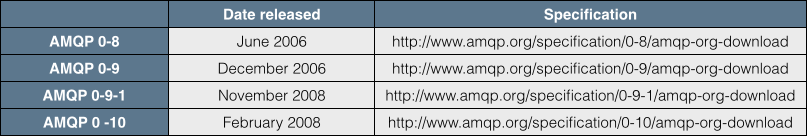
\includegraphics[scale=.5]{amqp_versions}  
\caption{Table of AMQP versions }
\label{Figure 1}  
\end{figure}

%In June 2006 - AMQP version 0-8 was released. - http://www.amqp.org/specification/0-8/amqp-org-download
%In December 2006 - AMQP version 0-9 was released. - http://www.amqp.org/specification/0-9/amqp-org-download
%In November 2008 - AMQP version 0-9-1 was released. - http://www.amqp.org/specification/0-9-1/amqp-org-download
%In February 2008 - AMQP version 0-10 was released.  - http://www.amqp.org/specification/0-10/amqp-org-download
%JPMorgan Chase collaborated with Red Hat to develop the Apache Qpid MOM implementation.  Independently, RabbitMQ was developed by Rabbit Technologies as well as AMQP complient implementations by Microsoft and StormMQ.
%The working group expanded to include 23 companies, including: Bank of America, Barclays, Credit Suisse, Deutsche B$\ddot{o}$rse Systems, Goldman Sachs, Microsoft Corporation, Novell, Red Hat, VMware and others.
%The AMQP standard also defines message orientation, queuing, routing, reliability, and security.   AMQP also describes the wire-level format of the data so that any nodes that are AMQP compliant can handle the message stream.  
%Standardization lead to the rapid development of many MOM systems such as: Apache Qpid, RabbitMQ, StormMQ, ActiveMQ, Apache Apollo, SwiftMQ.  Even Microsoft supports the AMQP1.0 protocol with their implementation of the ServiceBus class in .NET  and is a supported protocol on the Azure cloud computing platform.  
%MOM implementations that support the AMQP version 1.0 specification (Released October 29th 2012) \cite{todo} are interoperable and are available on many platforms.  

AMQP 1.0 was released by the AMQP working group on October 30th 2011.  The next day, on November 1st 2011, the AMQP working group announced its reorganization as a OASIS member section. \cite{AMQP}

\section{AMQP 1.0}

AMQP is a layered protocol.  The first layer defines a type system and a set of encodings that must be used to represent fundamental types.  The second layer defines an binary, peer-to-peed protocol for transporting messages between two nodes on a network.  Layer three defines the overall AMQP message format, its contents and header/footer structure.  Layer four defines a communication protocol and how to atomically cluster messages.  Layer five deals explicitly with security, which from the ground up is a fundamental part of AMQP \cite{AMQP1.0}. 

\missingfigure[figwidth=6cm]{Diagram of AMQP layers}
\todo{Use O'Hara's diagram as a guide}

AMQP treats all nodes equally - it places no constraints on roles of connections endpoints.   Because of historical reasons most AMQP messaging systems are broker centric - client nodes connect to a centralized message passing mechanism to exchange messages.  At the most fundamental level a broker is a trusted intermediary, in the AMQP model a broker has three primary responsibilities \cite{UNKNOWN}:

%todo - work on citation information for this one...

\begin{enumerate}
\item Taking responsibility for messages sent by clients.
\item Co-ordinating client transactions.
\item Routing and distributing messages 
\end{enumerate}

\missingfigure[figwidth=14cm]{Diagram of Broker network}

\subsection {Specific differences}

AMQP 1.0 is a major departure from earlier AMQP versions.  While it imposes far fewer semantic requirements, the protocol is substantially more complex \cite{RABBITMQ_PROTOCOLS}.  Pre AMQP 1.0 versions specify both a  wire-level protocol and a broker architecture.  AMQP 1.0 only specifies a protocol and does not impose any architecture model on implementations \cite{REDHAT1}.

AMQP 1.0 is a symmetric protocol, all nodes are treated equally.  Earlier versions are asymmetric, each connection must have a defined client and broker.  This allows for broker-less point-to-point connections to be made using AMQP 1.0, where as every connection in Pre AMQP 1.0 versions were required to have at least one broker between clients.  AMQP versions before 1.0 also specified protocol commands to manage brokers.  AMQP 0-10 specifies commands such as "Create Queue", "Delete Queue", etc.  AMQP 1.0 does not define these messages as part of the protocol and assumes that this functionality will be part of each specific implementation.  \cite{REDHAT1} 
Previous AMQP versions had strict definitions for clients and brokers.  Every connection must have a defined client and server (broker).  The AMQP 1.0 standard is much more flexible, it permits point-to-point connections where no central broker or broker network is part of the data transfer.  

\subsection{backwards capability}

AMQP 1.0 is not backwards compatible with earlier AMQP versions.  

\subsection{Backlash to AMQP 1.0}

The release of AMQP 1.0 is not without controversy.  The 1.0 was a major departure from the previous AMQP versions and caused significant backlash among the AMQP community.  At least two of the major players in the AMQP working group have decided not to implement the 1.0 standard.  Even two years after the formal adoption of the AMQP 1.0 specification RabbitMQ does not directly support the AMQP 1.0 standard.  iMatix, one of the original members of the AMQP working group has moved away from the AMQP standard all together and now develops a competing messaging system $\emptyset$MQ \cite{ZERO_MQ}. 

\section{AMQP Alternatives}
The AMQP specification is not unique in its goal of providing a cross-platform, ubiquitous message protocol.  There are several popular specifications in current use.  Many MOM implementations that support the AMQP protocol also support these other protocols; some are built in natively while others need to be enabled as plugins.   

\subsection{STOMP}
Simple Text Oriented Message Protocol (STOMP) is a text-based protocol designed to work with message oriented middleware systems.  It defines a wire-level message encoding format that allows for STOMP clients to communicate with any STOMP enabled message broker.  It is built on top of TCP/IP and uses a protocol similar to HTTP \cite{STOMP}.

\subsection{OpenWire}
OpenWire is a binary protocol used as the native wire format of ActiveMQ \cite{OPENWIRE}.

\subsection{Extensible Messaging and Presence Protocol (XMPP)}
XMPP is a communications protocol based on XML.  Originally developed by the open-source community for instant messaging, presence information and contact list maintenance \cite{XMPP}  

\subsection{MQTT}
MQ Telemetry Transport (MQTT) is a light-weight messaging protocol.  It is specifically targeted for applications where a light-weight protocol is needed due to code size limitations.  The protocol was invented by Andy Stanford-Clark (IBM) and Arlen Nipper (Cirrus Link Solutions).  In 2013 the MQTT protocol specification was submitted to the OASIS specification body.  There is a variation of the standard (MQTT-S) for embedded applications on non-TCP/IP networks such as ZigBee.  Facebook Messenger uses the MQTT protocol internally for large parts of its functionality \cite{MQTT}. 

\subsection{Java Messaging Service (JMS)}
The Java EE JMS (Java Messaging Service) was the starting point for attempting to standardize MOM. Unfortunately, JMS only specifies an application programming interface (API) and does not specify a format for exchanged messages so it does not create interoperability.   To achieve this desired interoperability other standards such as AMQP (Advanced Message Queuing Protocol) built upon the JMS standards). 

\section{AMQP implementations}

\subsection{Broker implementations}

There are several major open source AMQP broker implementations.  

\begin{figure}
\centering
\vspace{2.0in} 
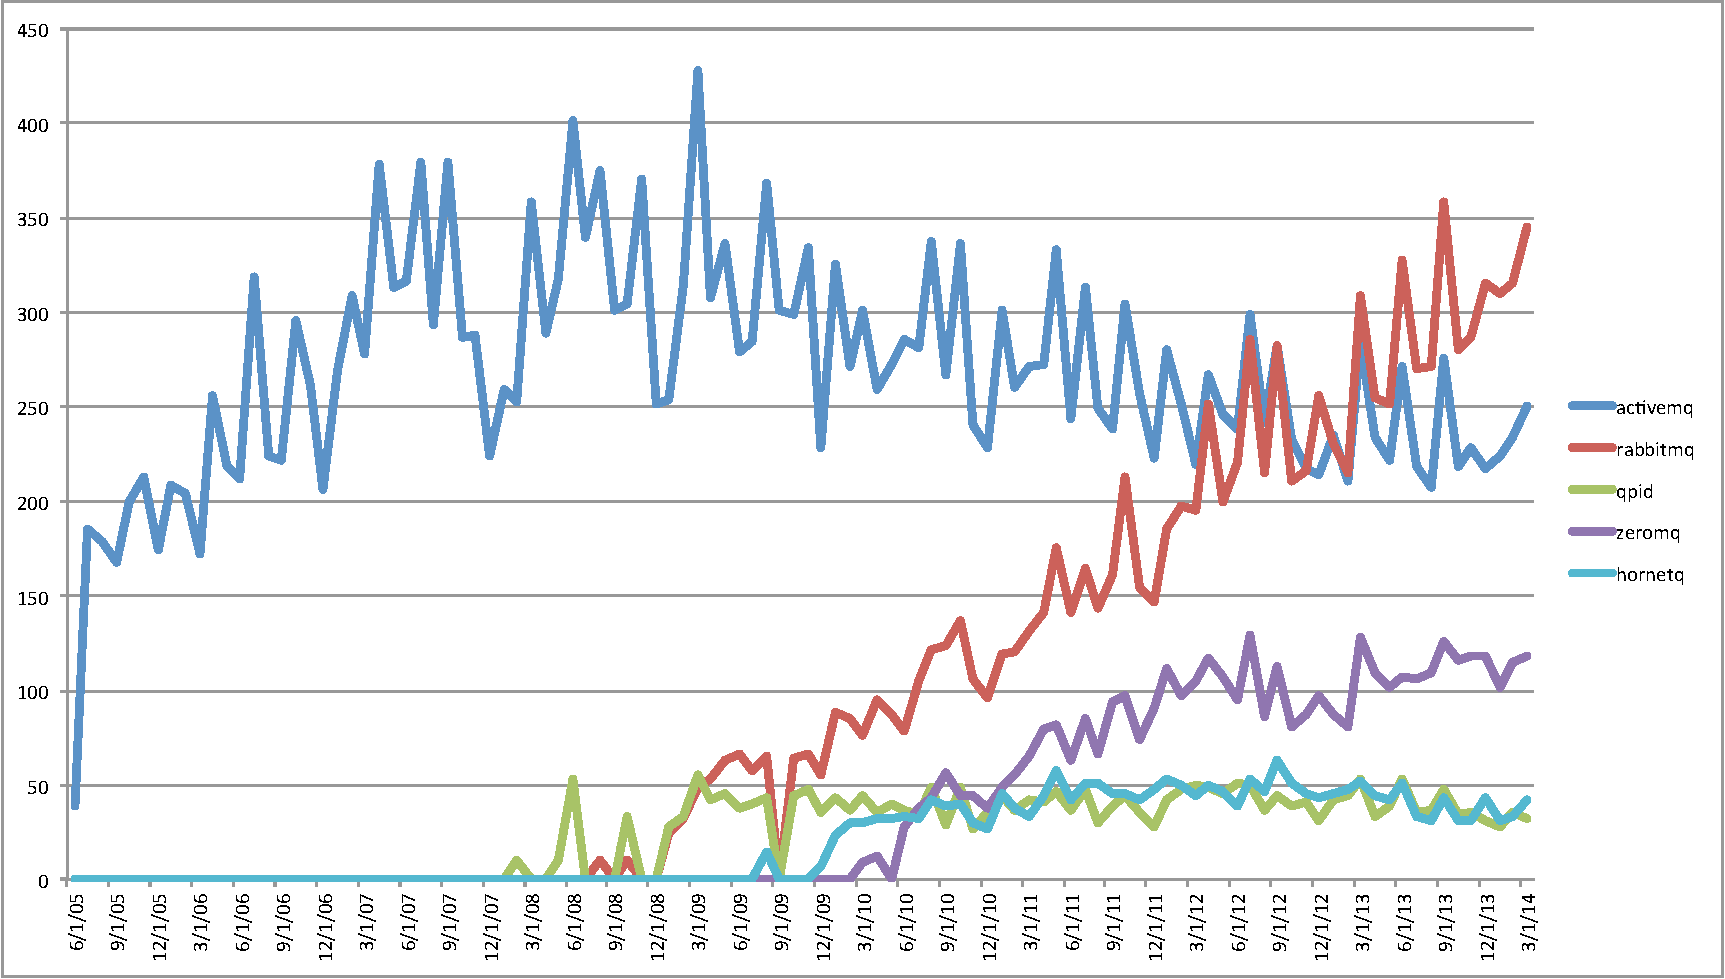
\includegraphics[scale=.5]{broker_popularity}  
\caption{Google trend data for AMQP implementations}
\label{Figure 1}  
\end{figure}


\subsection{RabbitMQ}
RabbitMQ is an open source message broker written in the Erlang programming language \cite{RABBITMQ} RabbitMQ is developed by and supported by Rabbit Technologies Ltd.  It is actively being developed, the latest stable version (3.2.4) was released on March 4, 2014.  It is licensed under the Mozilla Public License \cite{rabbitmq-wikipedia}.  The development history/management of RabbitMQ is complicated.  Originally developed by Lshift, the project was moved to an independent company Rabbit Technologies Ltd, which was cofounded by Monadic and CohesiveFT.  In 2013, Rabbit Technologies Ltd. was acquired by SpringSource, a division of VMware, Inc. \cite{LSHIFT}.  As of March 2014 - commercial support for RabbitMQ was being provided by Pivotal, Ltd \cite{PIVOTAL}.  RabbitMQ is cross platform and has bindings/clients for a wide range of systems/programming languages \cite{RABBITMQ_CLIENTS}.  

%has bindings/client for many different languages.  RabbitMQ has comprehensive documentation, and supports Clustering, High Availability, SSL, Management, etc. \todo{complete}

\subsection{ActiveMQ}
ActiveMQ is an open source message broker written in Java.  ActiveMQ is developed by the Apache Software Foundation and as of the writing of this report the most recent stable version is 5.9.0 released on October 21, 2013.  ActiveMQ is part of Apache's enterprise service bus (ESB) implementations, and is leveraged in other project such as Apache Camel and Apache CXF to Service Orientated Architecture (SOA) projects. Version 5.3 of Apache ActiveMQ has published performance results using the SPECjms2007 benchmark \cite{ACTIVEMQ_WIKI}. 

\subsection{ApolloMQ}
ApolloMQ is an open source message broker written in Java.  It is a fork of Apache ActiveMQ with the primary difference being the threading model and message dispatching architecture.  ApolloMQ maintains multi-protocol support and supports STOMP, AMQP 1.0, MQTT, OpenWire, SSL and WebSockets \cite{APOLLO}.

\subsection{HornetQ}
HornetQ is an open source, multi-protocol messaging system developed from JBoss, a division of Red Hat, Inc. \cite{REDHAT}.  It can be integrated with JBoss Application Server or embedded into standalone applications.  As of version \todo{find version} it supports the AMQP1.0 specification.  HornetQ is released under the Apache Software License version 2.0 \todo{citation needed}.  There are a few components that are released under LGPL \todo{citation needed} but the plan is to develop a pure ASL2.0 version in the future.  HornetQ is written in Java and supports and platform with a Java 5 or later runtime.   It is actively being developed and maintained with the last stable version 2.4.0 being released on December 16, 2013. \cite{HORNETQ}.  As of 4/10/2014 HornetQ holds the SPECjms2007 benchmark record \cite{HORNETQ_WIKI}.

\subsection{Client implementations}
There are many different AMQP client libraries for connecting a software components to an AMQP broker.  There are ports for most programming languages, for example RabbitMQ lists 175 different client libraries for over 21 different programming languages \cite{RABBITMQ_CLIENTS}

The maturity and functionally for each client vary greatly.  Granted, many of the client libraries are open source and have low activity, but there are several open source client libraries with active support.  There are also closed source, proprietary implementations and while they may be free to use there are license restrictions that make them unusable for this project \footnote{Specificially SwiftMQ has a clause in their license that prohibits publishing benchmarking results without company approval} One of the most active and widely used client libraries is Apache's Qpid Proton library \cite{QPID_PROTON}, which has both C and Java implementations.  

\begin{figure}
\centering
\vspace{2.0in} 
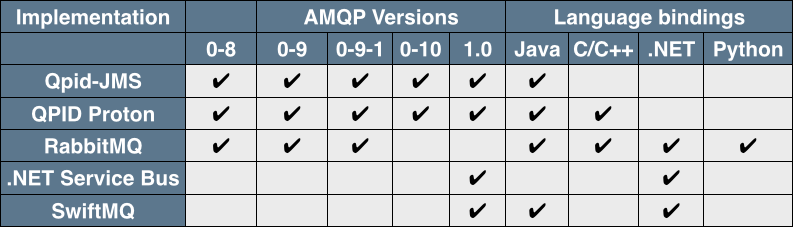
\includegraphics[scale=.5]{client_comparision}  
\caption{Summary of available AMQP clients}
\label{Figure 1}  
\end{figure}

\chapter{Methodology}
There are three independent steps for generating the testing data for this project.  Each step will be completed independently using the same lab setup, computing hardware and software.  As much as possible outside factors will be minimized to help ensure that the collected data is comparable.  AMQP brokers are complicated software components, with many interacting parts so care must be taken to ensure that the data collected is reliable.  

For the first step baseline performance data will be collected on the performance of each AMQP broker implementation in isolation.  There have been many experiments run with this configuration \cite{BENCHMARK1} \cite{BENCHMARK2}.  While this step is not novel it will allow us to compare results with independent AMQP evaluations to ensure that the developed benchmark produces reliable results. 

The second step for this project is to create simple broker networks of homogenous AMQP broker implementations and collect benchmark information.  The broker network configurations will follow the designs described by  Marsh, Sampat, Potluri, Panda in \cite{Scaling AMQP} so that this data may again be compared to an independent evaluation to ensure that the collected results are valid.

The third and final step is to create heterogeneous broker networks using the same broker network architecture in step two.  This will allow for direct comparison of the impact of integrating different AMQP broker networks into a single system.  This will model one of the goals of the AMQP working group and will provide meaningful, real world data on the interoperability and performance of the AMQP broker implementations. 

\todo{Section describing Networking benchmark background}


\section{Hardware setup}
A lab environment will be setup to isolate the tests from outside message traffic.  High-end workstation, class laptop computers and business class network equipment will be used.  The computers will use the latest Long-Term Support version of the Ubuntu Server operating system (12.04LTS) and will be configured to minimize background daemons and processes.  The times of all systems will be synchronized using a local NTP server. A complete listing of software versions used will be published with the results of this research.

\subsection{Network design}


\section{Benchmark design}

The design of the benchmarks for this experiment we modeled after the work done by Subramoni, Marsh, Narravula, Lai and Panda in \cite{Subramoni} which in turn based their benchmarks on Ohio State University Micro-benchmarks \cite{OSU_MICRO_BENCHMARKS}.

\subsection{Existing Benchmarks}
There are other existing and published benchmarks for MOM systems.  The most widely known is SPECjms2007 \cite{SPEC_JMS2007}.  It was the first industry standard benchmark for evaluating the Java Messaging Service (JMS).

SPECjms2007 is designed to model a messaging system of a grocery store - it simulates all of the messages needed to maintain inventory/purchasing/etc.  It does this to provide a comprehensive - real-world evaluation of a messaging system.  The benchmark was expanded by \todo{find name and reference} to originally benchmark the Apache Qpid MOM system \cite{citation needed}.  The benchmark needs to be licensed from the SPEC organization.  


\subsection{Format of test data}


%Each step is setup to collect meaningful data about the performance of each AMQP broker implemenation

 %developed broker network architectures and benchmarked to support large federated broker networks and benchmarked the messaging passing performance.  They experimented with multi-level broker architectures and multi-consumer fanout patterns to find the optimal broker design patterns.  All of their work was performed with Apache Qpid implementation [3].  

%Subramoni, Marsh, Narravula, Lai and Panda in [1] designed and developed benchmarks for MOM broker networks building using the Message Passing Interface (MPI) benchmarks developed by Ohio State University Network-Based Computing Laboratory’s [1] and the Standard Performance Evaluation Corporation (SPEC) MOM benchmarks  [1].  Benchmarks such as the Direct Exchange - Single Publisher Single Consumer (DE-SPSC) and Direct Exchange - Multiple Publishers Multiple Consumers (DE-MPMC) benchmarks [1] will be implemented for each AMQP implementation 

%This project will combine the methodologies used in these experiments and add an additional variable, different broker implementations to determine what the performance impact of a heterogenous broker network on messaging performance.

%In addition to these benchmarks, additional information will be collected in order to compare the performance of the broker implementations.


\begin{figure}
\centering
\vspace{2.0in} 
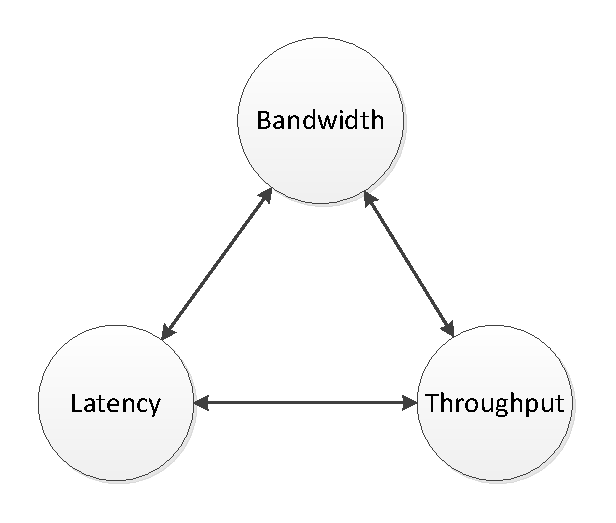
\includegraphics{bandwidth_latency_throughput}  
\caption{Relation between bandwidth, latency and througput}
\label{Figure 1}  
\end{figure}


Because these implementations were designed around the message traffic of the financial services sector they excel at passing small messages and focus on message throughput.  There are performance differences between each implementation and generic benchmarks for each implementation are available \cite{todo}\cite{todo}.

\begin{figure}
\centering
\vspace{2.0in} 
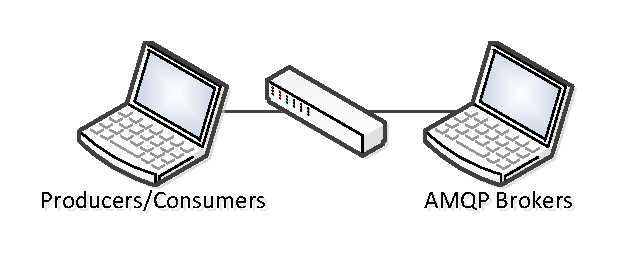
\includegraphics{test_setup}  
\caption{Test setup overview}
\label{Figure 1}  
\end{figure}



\subsection{Direct Exchange - Single Publisher Single Consumer (DE-SPSC)}

\begin{figure}
\centering
\vspace{2.0in} 
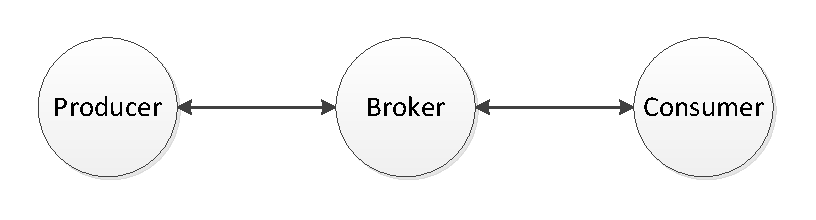
\includegraphics{direct_connect}  
\caption{Direct Exchange - Single Publisher Single Consumer (DE-SPSC)}
\label{Figure 2}  
\end{figure}

\subsection{Direct Exchange - Multiple Publishers Multiple Consumers (DE-MPMC)}

\subsection{Single Publisher - Multiple Consumer (SPMC)}

\begin{figure}
\centering
\vspace{2.0in} 
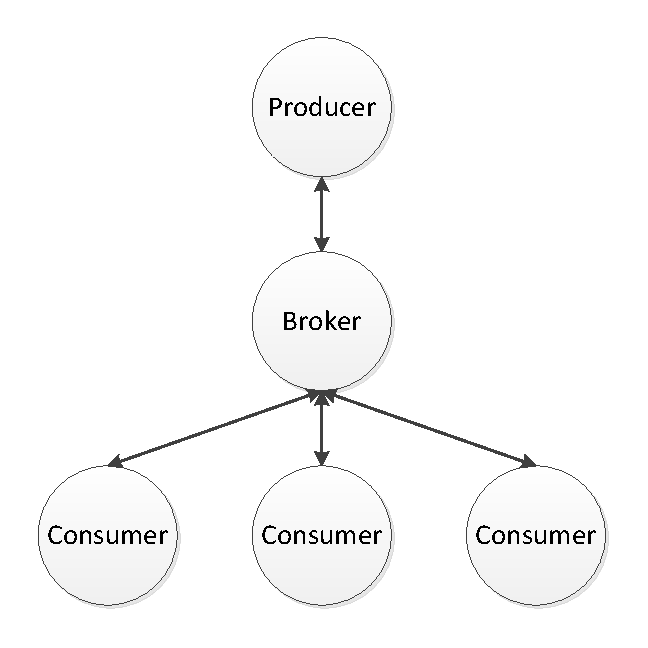
\includegraphics{simple_fanout}  
\caption{Single Publisher - Multiple Consumer (SPMC-S)}
\label{Figure 3}  
\end{figure}

\begin{figure}
\centering
\vspace{2.0in} 
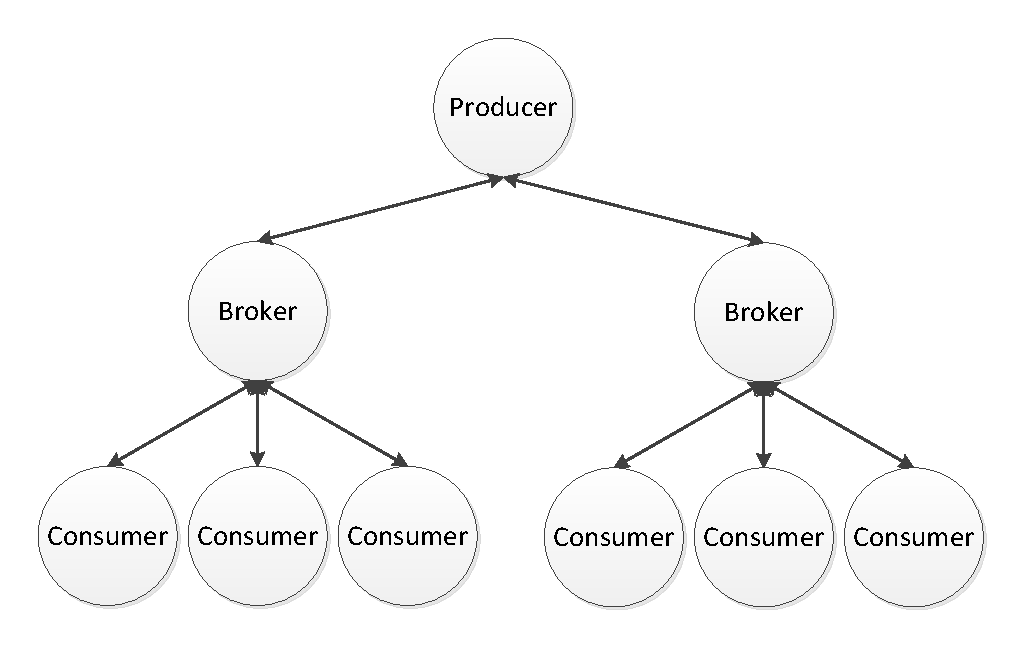
\includegraphics{complicated_fanout}  
\caption{Complex - Single Publisher - Multiple Consumer (Complex)(SPMC-C)}
\label{Figure 4}  
\end{figure}

\subsection{Topic Exchange - Single Publisher Single Consumer (SPSC)}


\chapter{Experimental Results}

From the beginning of the project creating a simple AMQP producer and consumer proved to be more difficult than expected.  Even though all of the AMQP broker implementations chosen to benchmark claim to support AMQP 1.0 each of them required more work than anticipated to get data flowing.  

Apache ActiveMQ worked out of the box.  
Apache Apollo needed additional client library calls before clients could exchange data.
Apache Qpid 
RabbitMQ was a nonstarter.  While they claim to have an AMQP 1.0 plugin to enable the protocol on their broker implementation, no amount of configuration of either the broker or the client resulted in a working message passing instance.  Investigation into the issue revealed that in spite of adding and enabling the AMQP 1.0 plugin to RabbitMQ the broker was identifying the underlying transport as 0-9-1.  Frustratingly, although the Qpid JMS Client library also claimed to be configurable to support AMQP 0-9-1 no amount of client side configuration or modification of the benchmark software resulted in a viable message passing system.
It was a similar experience with HornetQ, which claims to have native AMQP 1.0 support. 

%\subsection{Experimental Setup}
%And so on, for more chapters.
%Another citation for the bibliography:\cite{anotherbook}
%
%  This is a sentence to take up space and look like text.
%   This is a sentence to take up space and look like text.
%   Please refer to Figure~\ref{Figure 1}.  % Note \label command below

%\begin{table}
%\caption{This is the Caption for Table 2}
%\label{mytable}
%\begin{center}
%\begin{tabular}{lll}
%Here's	& another 	& example \\
%of		& something	& useful \\
%\verb+table+ & environment & command. \end{tabular}
%\end{center}
%\end{table}

% The following produces a numbered bibliography where the numbers
% correspond to the \cite commands in the text.
\specialhead{LITERATURE CITED}
\begin{singlespace}
\begin{thebibliography}{99}

\bibitem{ActiveMQ} B. Snyder, D. Bosanac, R. Davies, "ActiveMQ in Action", Manning, 2011 pp 1 – 326.

\bibitem{Scaling AMQP} G. Marsh, A. Sampat, S. Potluri, D. Panda, "Scaling Advanced Message Queueing Protocol (AMQP) Architecture with Broker Federation and InfiniBand", Department of Computer Science and Engineering, The Ohio State University

\bibitem{Chirino} H Chirino, "STOMP Messaging Benchmarks: ActiveMQ vs Apollo vs HornetQ vs RabbitMQ", http://hiramchirino.com/blog/2011/12/stomp-messaging-benchmarks-activemq-vs-apollo-vs-hornetq-vs-rabbitmq/

\bibitem{Sachs} K. Sachs, K. Samuel, and S. Appel, "Benchmarking of Message-Oriented Middleware", ACM, pp. 1–2, Sep. 2009.

\bibitem{Subramoni} H. Subramoni, G. Marsh, S. Narravula, P. Lai, D. Panda, "Design and Evaluation for Financial Applications using Advanced Message Queuing Protcol (AMQP) over InfiniBand", Department of Computer Science and Engineering, The Ohio State University.

\bibitem{Maheshwari} P. Maheshwari and M. Pang, “Benchmarking Message-Oriented Middleware – TIB/RV vs. SonicMQ,” Journal Concurrency and Computation: Practice and Experience - Foundations of Middleware Technologies, vol. 17, no. 12, pp. 1507–1526, Oct. 2005.

\bibitem{OASIS} "OASIS Homepage", https://www.oasis-open.org/org

\bibitem{WIKI_OSI} http://en.wikipedia.org/wiki/OSI_model

\bibitem{ORACLE_JMS} http://docs.oracle.com/javaee/6/tutorial/doc/bncdq.html

\bibitem{Kramer} Joshua Kramer, "Advanced Message Queueing Protocol (AMQP)", Linux Journal, Nov. 2009, http://www.linuxjournal.com/magazine/advanced-message-queuing-protocol-amqp

\bibitem{O'Hara} “Toward a Commodity Enterprise Middleware: Can AMQP Enable a New Era in Messaging Middleware? A Look Inside Standards-Based Messaging with AMQP”, http://queue.acm.org/detail.cfm?id=1255424

\bibitem{Hintjens} "What is wrong with AMQP, http://www.imatix.com/articles:whats-wrong-with-amqp/

\bibitem{OPEN_AMQ} "Homepage", http://www.openamq.org/

\bibitem{QPID_HOMEPAGE} http://qpid.apache.org/

\bibitem{Apps, Cameron} J. Apps, B. Cameron, "AMQP and RabbitMQ - Message Queueing as an Integration Mechanism", http://www.openvms.org/skonetski/Webinar_2012_09_AMQP_RabbitMQ_Message_Queuing_as_Integration_Mechanism.pdf

\bibitem{AMQP} http://www.amqp.org/node/54

\bibitem{AMQP1.0} http://docs.oasis-open.org/amqp/core/v1.0/amqp-core-complete-v1.0.pdf

\bibitem{Freeman} Freeman, E. (1996). Middleware: Link everything to anything. Datamation, 42(16), 119-119. Retrieved from http://search.proquest.com/docview/220221663?accountid=37764

\bibitem{UNKNOWN} http://www.rabbitmq.com/wp-uploads/2010/11/amqp-broker-prototype.pdf

\bibitem{BENCHMARK1} http://stackoverflow.com/questions/7921324/performance-comparison-between-zeromq-rabbitmq-and-apache-qpid

\bibitem{BENCHMARK2} , http://predic8.com/activemq-hornetq-rabbitmq-apollo-qpid-comparison.htm

\bibitem{REDHAT1} https://access.redhat.com/site/documentation/en-US/Red_Hat_Enterprise_MRG/2/html/Messaging_Programming_Reference/Differences_between_AMQP_0-10_and_AMQP_1.0.html

\bibitem{MQTT} http://en.wikipedia.org/wiki/MQ_Telemetry_Transport

\bibitem{RABBITMQ} http://www.rabbitmq.com

\bibitem{RABBITMQ_CLIENTS} http://www.rabbitmq.com/devtools.html

\bibitem{RABBITMQ_PROTOCOLS} http://www.rabbitmq.com/protocols.html

\bibitem{SPEC_JMS2007} http://www.spec.org/osg/jms2007/

\bibitem{OSU_MICRO_BENCHMARKS} http://mvapich.cse.ohio-state.edu/benchmarks

\bibitem{QPID_PROTON} http://qpid.apache.org/components/messenger/index.html

\bibitem{ZERO_MQ} http://zeromq.org/

\bibitem{HORNETQ} http://www.jboss.org/hornetq

\bibitem{REDHAT} http://en.wikipedia.org/wiki/JBoss_(company)

\bibitem{XMPP} http://en.wikipedia.org/wiki/XMPP

\bibitem{STOMP} http://stomp.github.io/

\bibitem{HORNETQ_WIKI} http://en.wikipedia.org/wiki/HornetQ

\bibitem{ACTIVEMQ_WIKI} http://en.wikipedia.org/wiki/ActiveMQ

\bibitem{OPENWIRE} http://en.wikipedia.org/wiki/OpenWire_binary_protocol

\bibitem{LSHIFT} http://www.lshift.net/blog/2010/04/13/rabbitmq-2

\bibitem{PIVOTAL} http://www.gopivotal.com/support 

\bibitem{APOLLO} https://activemq.apache.org/apollo




\todo{Not sure if I really want to advertise this. How on Earth am I going to actually support this}
NOTE: Printed copies of all sources are available upon request. 

\end{thebibliography}
\end{singlespace}


%%%%%%%%%%%%%%%%%%%%%%%  For Appendices  %%%%%%%%%%%%%%%%%%%
\appendix    % This command is used only once!
\addtocontents{toc}{\parindent0pt\vskip12pt APPENDICES} %toc entry, no page #
\chapter{THIS IS AN APPENDIX}
Note the numbering of the chapter heading is changed.
This is a sentence to take up space and look like text.
\section{A Section Heading}
This is how equations are numbered in an appendix:
\begin{equation}
x^2 + y^2 = z^2
\end{equation} 

\chapter{THIS IS ANOTHER APPENDIX}
This is a sentence to take up space and look like text.

\end{document}
